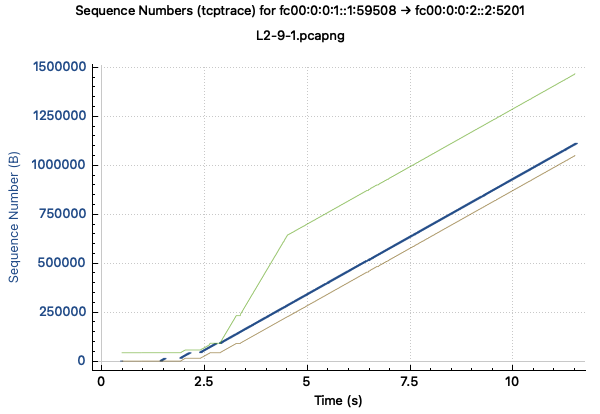
\includegraphics{Lab2/traces/tcptrace.png}

In Wireshark's TCP graph, blue indicates data sent, green shows data acknowledged, and orange represents duplicate acknowledgments due to out-of-order packets.
TCP's slow start phase gradually increases the sender's rate until congestion occurs. The graph displays a sawtooth pattern, with the blue line representing the sending rate increasing and decreasing as congestion is detected and resolved.

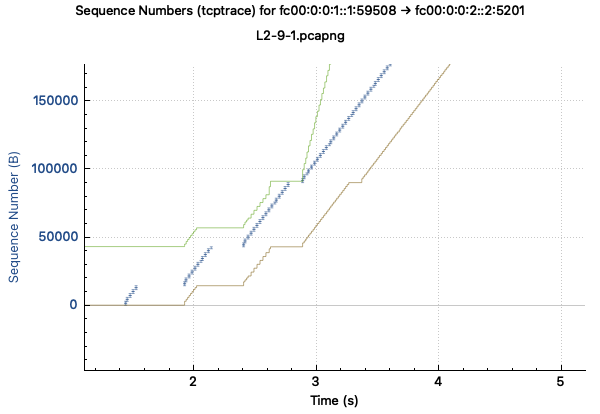
\includegraphics{Lab2/traces/exponenential.png}